In this section, after discussing the assumptions and system model, the problem of joint SFC deployment and VNFM placement is stated and clarified by an illustrative example.

\subsection{Assumptions}\label{assumptions}
In the JSD-MP problem, a set of SFCs need to be deployed in the physical infrastructure network.
The main assumption is that in addition to computational and network resources,
a VNFM should be assigned for each SFC to manage the VNFs of the SFC.
All VNFs of a chain should be managed by a single VNFM, but a VNFM can manage multiple SFCs.
The capacity of each VNFM is limited in terms of the number of VNF instances.
Each VNFM needs a license for managing the specific number of VNF instances.
Moreover, we assume that only a subset of physical servers can host VNFs and similarly,
each VNF type can only be placed on a subset of physical servers,
as an example ingress and egress type of functions need to be placed on ingress and egress nodes respectively.
VNF instances deployed on a physical server can only be managed by the VNFMs placed on a given subset of physical servers.
To maintain the timing requirement of management traffic,
the distance (in term of hop-count) between each VNFM and its associated VNFs should be less than the specified threshold.
Also, JSD-MP considers VNFs can't shared between chains.
Only a subset of VNF types need to managemed an other can be deployed without an assigned VNFM.

\subsection{System Model}
% parameters will define here and decision variables will defined in formulation section.
%
%% Infrastructure's parameters have superscript "p"
%% Chain's parameters have superscript "s"
%% Infrastructure's nodes have subscript "i", "j"
%% Chain's nodes have subscript "u", "v"
%% Use parentheses for functions and in rare occasions
%% Management's parameters have superscript "m"
%% Use capital letters for sets
%

The physical infrastructure topology is modeled as a directed graph \(G^p=(V^p, E^p)\),
where \(V^p\) is the set of NVFI-PoPs and \(E^p\) is a set of the inter-PoP links.
The computational capacity of PoP \(i \in V^p\) is specified by \(c^p_i\) number of CPU cores and \(m^p_i\) gigabytes of RAM.
Bandwidth of link \((i,j) \in E^p\) is specified by \(b^p_{(i.j)}\).

The set of requested SFCs is denoted by \(R\).
Each request \(h \in R\) has revenue \(c_h\) and
is represented by directed graph \(G^s_h = (V^s_h, E^s_h)\),
where \(V^s_h\) is the set of VNFs of the chain and \(E^s_h\) is the set of the virtual links of the chain.
The type of VNF \(v \in V^s_h\) is denoted by \(t_{v,h} \in T\).
Each type \(k\) determines the required number of CPU cores \(c^s_k\)
and the required amount of memory \(m^s_k\) to create an instance of that type.
The required bandwidth of each virtual link \((u,v) \in E^s_h\) is denoted by \(b^s_{(u,v),h}\).
Each VNFM requires \(c^m\) number of CPU cores and \(m^m\) gigabytes of RAM to handle \(\kappa\) number of VNFs at most.
To have better quality in management each VNFM reserves \(b^m\) bandwidth per management link.
Lunching VNFMs requires to have license for each instance by cost \(\phi\).
we will use \(\phi\) to indicate the maximum hop counts for management,
\(\eta_{(i, j)}\) indicates that physical server \(i \in V^p\) can manage \(j \in V^p\).
\(\omega_k\) indicates that type \(k \in T\) requires manager or not.
\(\psi_i\) indicates that physical server \(i \in V^p\) support VNFs or not.

The notations used in this paper are summarized in Table \ref{tbl:parameters}.

\subsection{Problem Statement}
Using the defined notations and under the assumptions of subsection \ref{assumptions},
the JSD-MP problem is defined as following. The NFVI service provider owns the infrastructure network \(G^p\).
A set \(R\)of requests are given. The service provider's goal is to accept a subset of requests that maximize the profit.
To accept a request \(h\), the service provider should allocate the \(c^s_{t_{v,h}}\) CPU core, and \(m^s_{t_{v,r}}\) amount of memory for all \(v \in r\),
\(b^s_{(u,v),h}\) bandwidth for all links \((u,v) \in E^s_h\) and a VNFM.
These allocations should satisfy the requirements mentioned in subsection \ref{assumptions}.
The profit is made by revenue obtained from accepting the requests while the service provider should pay the license cost of \(\phi\) for each VNFM.

The idea behind the JSD-MP problem is that in the placement of VNFM for a chain, the location of the VNFs of the chain should be taken into account.
Therefore, by jointly conducting of SFC deployment and VNFM placement, the service provider can maximize the profit.

This problem is clarified by an illustrative example in the following subsection.
% TODO: Reference the formulation and solution section.
It is formulated in Section ??? and solved in Section ???.

\subsection{Example}
\par
\hly{I will review it later}
In this example, we want to consider an illustrative example to gain more sight into JSD-MP problem.
Figure~\ref{fig:example-chains} shows request chains with their type and links. link required bandwidth are in Mbps.
The NFVI service provider owns the infrastructure that is shown in Figure~\ref{fig:example-topology}.
VNF's types are described in Table~\ref{tbl:example-vnf-types}.
Table~\ref{tbl:example-server-spec} describes the physical servers specifications.
Instances can only run on servers 1, 3, 5, and 7.
Servers 1 and 3 can only be managed by the servers 2 and 4.
Server 5 can only be managed by the servers 4 and 6.
Server 7 can only be managed by the servers 6 and 8.
Each VNFM can handles 5 instances with 4 GB of RAM and 2 CPU cores.
All physical links has 40Gbps capacity.

\begin{figure}
    \centering
    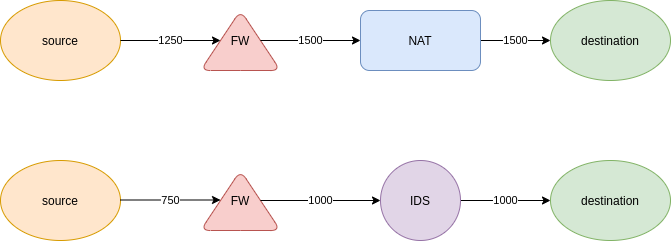
\includegraphics[height=150px]{images/example-chains.png}
    \caption{Chains for illustrative example}
    \label{fig:example-chains}
\end{figure}

\begin{figure}
    \centering
    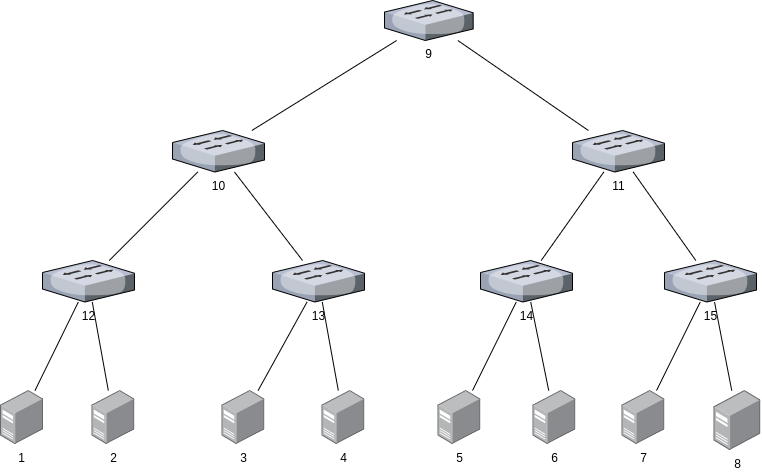
\includegraphics[height=150px]{images/example-toplogy.png}
    \caption{Topology of illustrative example}
    \label{fig:example-topology}
\end{figure}

\begin{table}
    \centering
    \caption{VNFs type of illustrative example}
    \begin{tabular}{|c|c|c|c|}
        \hline
        Spec/VNF & vFW & vNAT & vIDS \\
        \hline
        CPU (vCore) & 2 & 2 & 2 \\
        \hline
        Memory (GB) & 2 & 4 & 2 \\
        \hline
    \end{tabular}
    \label{tbl:example-vnf-types}
\end{table}

\begin{table}
    \centering
    \caption{Server specification of illustrative example}
    \begin{tabular}{|c|c|c|}
        \hline
        & Server 1,2,7,8 & Servers 3,4,5,6 \\
        \hline
        Installed vCPU & 144 & 72 \\
        \hline
        Installed Memory (GB) & 1408 & 288 \\
        \hline
        Link (Gbps) & 40 & 40 \\
        \hline
    \end{tabular}
    \label{tbl:example-server-spec}
\end{table}

\subsection{Importance}
\par
This problem considers VNFs and their requirements for management by a VNFMs.
Considerations in this problem tries to be realistic and be useful at data centers.